\documentclass[times, 10pt,twocolumn]{article}

\usepackage{sose2011}
\usepackage{times}
\usepackage{color}
\usepackage[pdftex]{graphicx}

\graphicspath{{./images/}}
\DeclareGraphicsExtensions{.pdf,.jpeg,.png,.jpg}

% correct bad hyphenation here
\hyphenation{op-tical net-works semi-conduc-tor}
\pagestyle{empty}

\begin{document}

\title{SWAMP: Software Assurance Marketplace}

\author{
        \textbf{Smitha Sam}\hspace*{0.1in}
        \textbf{James Obert}\hspace*{0.1in}
        \textbf{Christopher C. Lamb}\\
        Science \& Engineering Information Systems \\
        Sandia National Laboratories \\
        \small{\{ssam, jobert, cclamb\}@sandia.gov}
}

\maketitle
\thispagestyle{empty}

\begin{abstract}
abstract
\end{abstract}

{
\setlength{\parindent}{0mm}
\textbf{Keywords:} Intelligent Agents, System of Systems.
}

\section{Introduction}
The nation’s critical infrastructure, businesses, and utilities are extensively controlled and enabled by software. These software systems, and their associated hardware platforms, must perform in a predictable and reliable manner. As the complexity of software systems increase, the demands and sophistication of the techniques and tools necessary to test, evaluate, and demonstrate assurance also increase. The development of these tools and approaches is an area of ongoing and active research.  It has been noted that the research community could benefit from a facility architected such that access to securely configured and controlled hardware platforms, rules and vulnerabilities databases, and threat descriptions are readily available to the community in a real-time manner.

A federated test bed and analysis environment is proposed to facilitate the creation of new approaches and tools for software assurance activities. This test bed and analysis environment, referred to as a Software Assurance Marketplace (SWAMP) will provide both open source and proprietary services and infrastructure to test new assurance algorithms on software systems in heterogeneous environments with access to hardware ranging from desktop to high performance computing systems.   The SWAMP will be installed in a secure, isolated environment at Sandia to enable the evaluation of assurance techniques that need to be protected. 

This SWAMP will dramatically accelerate the development of assurance tools and techniques that can be quickly applied to critical software components and systems. It is expected that application of the advanced tools developed within the SWAMP will significantly raise software assurance levels, reduce costs, and positively impact critical infrastructure software throughout its lifecycle.

\begin{figure}[!t]
\centering
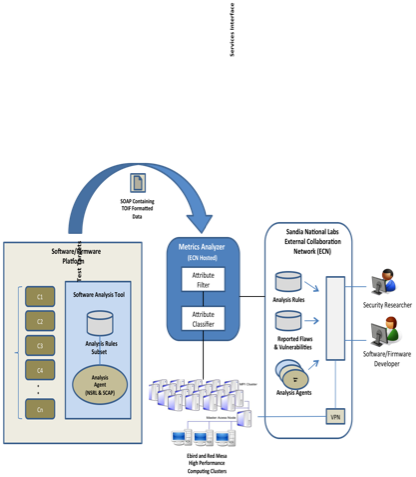
\includegraphics[width=3in]{image001}
\caption{Conceptual Architecture.}
\label{fig:con-arch}
\end{figure}  

\subsection{Previous Work}


\section{Technical Approach}\label{sec:tech}
Sandia National Laboratory’s primary mission is to maintain and provide failsafe nuclear weapon systems. In support of our mission a large number of software/firmware assurance modeling and simulation techniques and tools have evolved. Achieving failsafe assurance levels in our systems requires the use of extremely capable computing platforms executing complex modeling and simulation scenarios. One of many such systems available at Sandia is Red Storm consisting of 38,000 processor cores with an effective massively parallel processing speed of 204.2 TFLOPS. In addition to Red Storm, Sandia’s Service Oriented Architecture (SOA) contains a Core Enterprise web services platform offering federated secure web service capabilities in support of distributed test analysis agents and web based user interfaces. The following sections describe a high-level design for a Sandia hosted Software Assurance MarketPlace (SWAMP) that enables:

•	Research into new forms of software analysis and testing in secure, reliable and repeatable workflows.
•	Expansion into new forms of testing including static, dynamic, and binary analysis.
•	Compatibility as a plug-in to DHS specified software analysis tools.
•	Interoperability as specified by the Homeland Open Security Technology (HOST) program.        

\subsection{Sandia SWAMP Infrastructure}\label{sec:tech:infra}
The proposed Sandia SWAMP infrastructure as shown in the figure below provides web services and VPN interfaces such that security researchers, software developers, and other pertinent staff members are able to analyze collected test data, develop/configure analysis agents and data classifiers.       

\begin{figure}[!t]
\centering
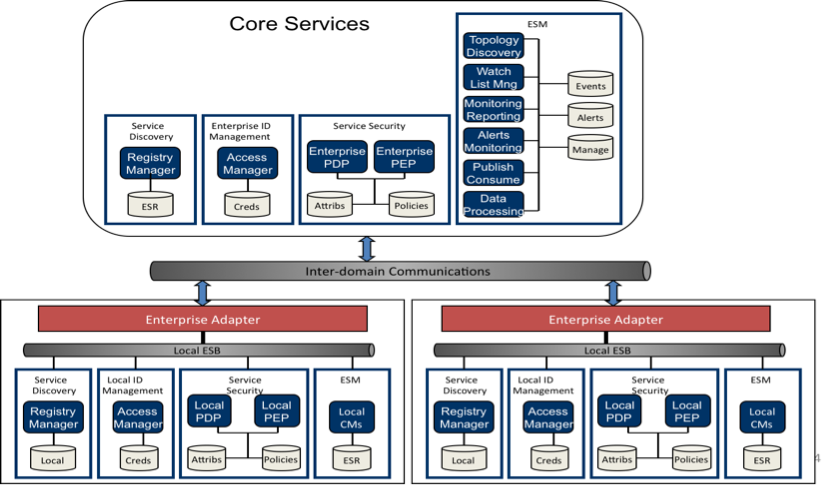
\includegraphics[width=3in]{image005}
\caption{Federated SOA Infrastructure.}
\label{fig:soa-infra}
\end{figure}  

% Figure 1 1: Sandia SWAMP Infrastructure
User access is provided on a 24 by 7 basis utilizing Sandia’s existing External Collaboration Network (ECN) which allows users to develop and configure deployable National Software Reference Library (NSRL) and Secure Content Automation Protocol (SCAP) compliant analysis agents as plug-ins to DHS designated software analysis tools. Access via the Sandia ECN also allows users to develop and configure data collection Attribute Filters and Classifiers within a central Metrics Analyzer. Deployed analysis agents utilizing a platform specific rules subset, collect test metrics, format the metrics into TOIF form and periodically transmits it via The Simple Object Access Protocol (SOAP) over HTTPS to the Metrics Analyzer. Analysis Agents software updates to target test platforms, and test data transmissions to the Metrics Analyzer are securely and reliably transmitted utilizing Sandia’s WS-SecureMessaging and WS-ReliableMessaging compliant Inter-domain messaging service as shown in the SOA Infrastructure diagram below. In order to ensure that all deployed Analysis Agents are up to date and properly recognized each is registered in a UDDI Enterprise Service Directory located at Sandia. Additionally, access control is maintained within each domain of the federated system via Service Security Policy Decision Points (PEP), and Policy Enforcement Points (PDP). All PDP and PEP decision and enforcement logic is stored in domain level WS-Security Policy repositories that map Individual access policies on a per Analysis Agent or system user basis.   

Figure 1 2: Sandia Federated SOA Infrastructure

\subsection{Analysis Agent}\label{sec:tech:aa}
As shown in the figure below, a master Analysis Rules database derived from standards, capabilities, and vulnerability databases (CVE, CWE, SAFES, NVD and CAPEC) is assembled and maintained by participating security research and development organizations. Research members of security organizations first perform comprehensive threat analysis of target test systems. The resulting threat analysis findings guide which rules are extracted from the master database and included in the subset deployed with the Analysis Agent.
     
\begin{figure}[!t]
\centering
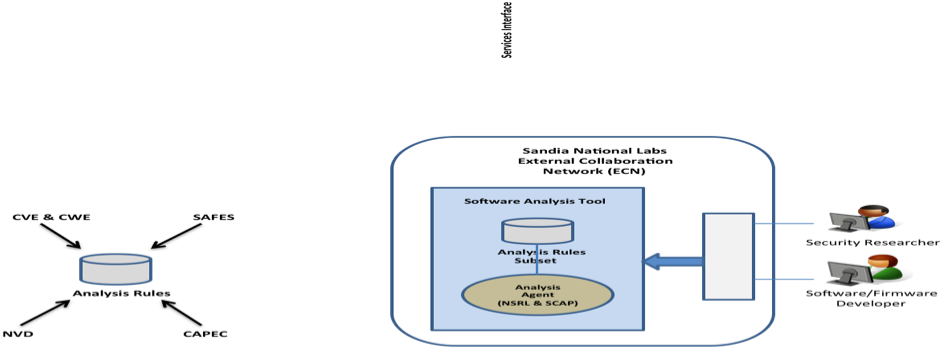
\includegraphics[width=3in]{image007}
\caption{Analysis Agent Configuration.}
\label{fig:aa-config}
\end{figure}  

Figure 1 3: Analysis Agent Configuration

Each Analysis Agent contains a rules interpreter capable of inspecting each rule and translating the rules into testing scripts native to the hosting software analysis tool. Each test scenario tests security-specific software architecture and design elements which effectively measure attack resistance, tolerance, and resilience.

\subsection{Metrics Analyzer}\label{sec:tech:ma}
The Metrics Analyzer consists of an Attribute Filter and Classifier which in combination are capable of parsing, trending and classifying the large amount of incoming Analysis Agent data. The Attribute Filter conditions Analysis Agent messages by removing message protocol constructs, and performing data compression. The Attribute Classifier uses machine learning and statistical methods to recognize specific software flaws and vulnerabilities. The classifier is capable of decomposing learning and statistical algorithms for parallel task execution on Sandia’s EBird and Red Mesa High Performance Clusters. Flaws and vulnerabilities identified during the classification process are stored in a database made available to security researchers through ECN hosted web services. 

\section{Conclusion}


\bibliographystyle{IEEEtran}
\bibliography{emr,drm}

\end{document}


